{\section{Ml-Agents}}
\label{sec:mlagents}
Das Unity ML-Agents Toolkit ist ein Open-Source-Projekt, in dem maschinelle Lernalgorithmen und Funktionen für die Verwendung mit der Spieleumgebung Unity implementiert und kontinuierlich weiterentwickelt werden. 

\subsection{Aufbau}
Die Implementierung ist in zwei Bereiche unterteilt. Für die Unity-Integration ist das Paket com.unity.ml-agents aus dem Unity Asset Store zuständig. Das eigentliche Training mit den maschinellen Lernalgorithmen findet jedoch in einer separaten Python-Umgebung statt. Für die Kommunikation zwischen den beiden Bereichen verwendet das ML-Agents Toolkit eine gRPC-Netzwerkkommunikation, worüber Zustand der Simulationsumgebung in Unity, ausgewählte Aktionen des neuronalen Netzes in Python und weitere Werte für die Auswertung des Trainings ausgetauscht werden.\cite{juliani2020}

\begin{figure}[H]
  \centering  
  \begin{tikzpicture}[node distance=2cm]
    \node(umgebung) [draw] {Umgebung};
    \node (agent1) [rounded, draw=green, fill=green!30, below of=umgebung, xshift=0.75cm, yshift=0.8cm] {Agent 1};
    \node (agent2) [rounded, right of=agent1, xshift=2cm, draw=green, fill=green!30] {Agent 2};
    \node (agent3) [rounded, right of=agent2, xshift=2cm, draw=green, fill=green!30] {Agent 3};
    \node (akademie) [rounded, below of=agent2 , draw=yellow, fill=yellow!30] {Akademie};

    \begin{pgfonlayer}{bg}
      \node(umgebung_bg) [draw, fill=black!20, inner sep=10pt, fit=(agent1) (agent2) (agent3) (akademie)] {};
    \end{pgfonlayer}

    \node (python_api) [rounded, below of=akademie, draw=orange, fill=orange!30] {Python API};
    \node (python_trainer) [rounded, right of=python_api, xshift=2cm, draw=red, fill=red!30] {Python Trainer};


    \draw [latex-latex, line width=0.3mm] (agent1)  |- node {} (akademie);
    \draw [latex-latex, line width=0.3mm] (agent2) -- (akademie);
    \draw [latex-latex, line width=0.3mm] (agent3) |- node {} (akademie);

    \draw [latex-latex, line width=0.3mm] (akademie) -- (python_api);
    \draw [latex-latex, line width=0.3mm] (python_api) -- (python_trainer);
  \end{tikzpicture}
  \caption{Unity ML-Agents Aufbau}
  \label{fig:mlagents_aufbau}
\end{figure}


Das Unity-Paket enthält drei Grundlegenden Komponenten, die Akademie, Agenten und Sensoren.
Das Unity-Paket enthält zwei Komponenten: Agenten und deren Verhalten. Die Agent-Komponente bildet die Grundlage für alle Implementierungen. Sie bietet abstrakte Funktionen für die Initialisierung, den Start einer Episode, das Erfassen des Zustands der Umgebung sowie das Ausführen von Aktionen. Durch die Implementierung dieser Funktionen können unterschiedlichste Agenten entwickelt und trainiert werden. Jeder Agent ist mit einem Verhalten verknüpft, das für jede Beobachtung des Agenten eine Aktion auswählt, die der Agent ausführt. Es gibt drei Arten, wie die Verhaltensweisen agieren können. Im Lernmodus werden die Beobachtungen des Agenten für das Training und die Auswahl einer Aktion anhand des aktuellen Modells verwendet. Der Inferenzmodus nutzt hingegen ein bereits trainiertes Modell und wertet dieses aus. Der letzte Modus eines Verhaltens ist der Heuristikmodus, bei dem festgelegte Regeln im Code entscheiden, welche Aktion ausgeführt wird, ohne die Verwendung eines trainierten Modells.\cite{juliani2020}

\subsection{Komponenten}
In diesem Kapitel werde Ich die Grundlegenden Komponenten des Unity ML-Agents Packets, welche in der Arbeit verwendet wurden erklären. Darurch sollten Codeausschnitte und Komponentenabbildungen in folgenden Kapiteln deutlich zu verstehen sein.

\subsubsection{Verhalten}
\begin{figure}[H]
  \centering  
  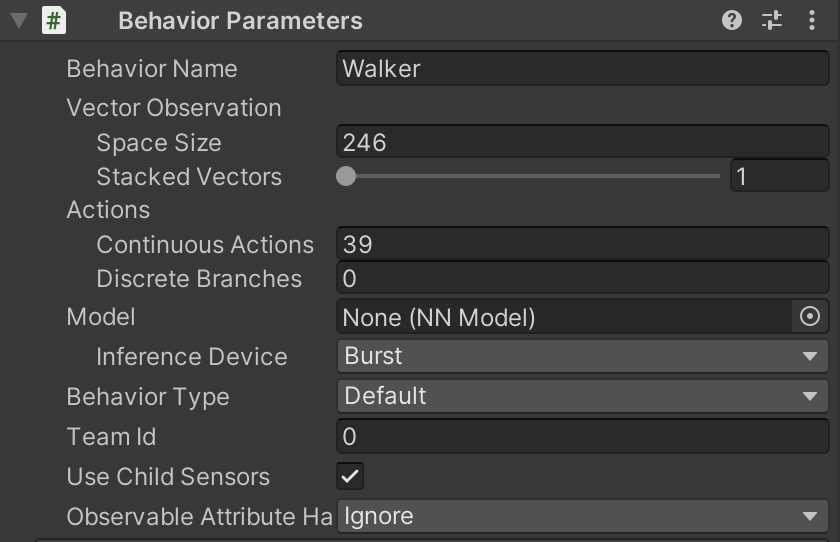
\includegraphics[scale=0.5]{img/verhalten_komponente.png}
  \caption{Unity ML-Agents Verhalten Komponente}
  \label{fig:verhalten_komponente}
\end{figure}

\begin{table}[H]
\centering
{\rowcolors{2}{lightgray}{gray!50!lightgray!50}
\begin{tabular}{ |p{4cm}|p{8cm}| }
\hline
Konfigurationsfeld& Beschreibung \\
\hline
Behaviour Name & Name des Verhaltens / wird in Trainer Konfiguration referenziert \\
Space Size & Anzahl an Beobachtungen / Inputknoten für NN \\
Continuous Actions & Anzahl an Aktionen / Outputknoten von NN \\
Model & Referenz auf bereits trainiertes Modell zur Verwendung in Inferenz \\
Behaviour Type & Lernmodus Default = Lernen, Heuristic, Inferenz \\
\hline
\end{tabular}}
\caption{Test}
\end{table}

\subsubsection{Entscheidung}
\begin{figure}[H]
  \centering  
  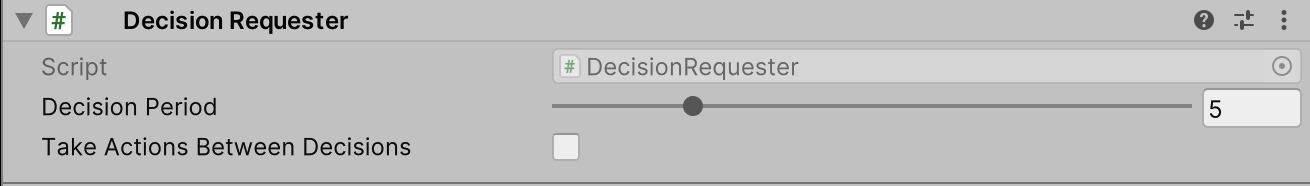
\includegraphics[scale=0.5]{img/entscheidung_anfragen_komponente.png}
  \caption{Unity ML-Agents Entscheidung Anfragen Komponente}
  \label{fig:entscheidung_anfragen_komponente}
\end{figure}

\begin{center}
{\rowcolors{2}{lightgray}{gray!50!lightgray!50}
\begin{tabular}{ |p{4cm}|p{8cm}| }
\hline
Konfigurationsfeld& Beschreibung \\
\hline
Decision Period & Anzahl an Akademie-Schritten (standard ein Schritt pro Physikupdate) bis zur nächsten Entscheidung \\
Take Actions Between Decisions &  Kontrollkasten ob Agent Aktionen zwischen Entscheidungen ausführen soll \\
\hline
\end{tabular}}
\end{center}


\subsection{Programmierschnittstellen}
\begin{lstlisting}[caption={Academy Instanzvariablen},captionpos=b]
envParams = Academy.Instance.EnvironmentParameters;
statsRecorder = Academy.Instance.StatsRecorder;
\end{lstlisting}
Die Akademie stellt mit dem Attribut EnvironmentParameters die Umgebungsparameter aus Trainer Konfiguration oder aktueller Lektion bereit

Mit dem StatsRecorder lassen sich Daten aggregieren um diese nach oder während dem Training über die Tensorboard Visualisierung auszuwerten

\begin{lstlisting}[caption={Agent Funktionen},captionpos=b]
public override void CollectObservations(VectorSensor sensor)
{
    sensor.AddObservation(floatObservation);
}

public override void OnActionReceived(ActionBuffers actionBuffers)
{
    var continuousActions = actionBuffers.ContinuousActions;
    float action = continuousActions[0]
}

public virtual void FixedUpdate()
{
    AddReward(floatReward);
}
\end{lstlisting}

In der CollectObservations Methoden wird festgelegt welche Daten dem Agent für das Training bereit stehen, dieser Schritt wird für jede angefragte Entscheidung ausgeführt und das Ergebnis an das NN Modell oder den Python Trainer übergeben.

Wenn eine Entscheidung angefragt wurde und das NN Modell ein Ergebnis liefert wird dieses hier von numerischen Werten in Aktionen umgewandelt.

Im folgenden Beispielcode wird ein Reward in jedem FixedUpdate vergeben über die AddReward Methode die auch Teil der Agenten-Komponente ist. Der Reward kann aber an jeder Stelle im Code vergeben werden, der Code dient hier nur als ein Beispiel.

Die Trainings Konfigurationdatei enthält mehrere Teile. Der hyperparameter Teil enthält die Hyperparameter des Maschinellen Lernalgorithmuses, danach folgt der network\_settings Teil welcher die Konfiguration des Neuronalennetzes festlegt. Anschließend folgen noch Konfigurationen für die Belohnungssignale im Bereich reward\_signals und Einstellungen für die Speicherung der Daten sowie der länge des Trainings. Ganz am Ende der Konfigurationsdatei befinden sich noch Umgebungsparameter welche erweitert und während dem Training ausgelesen werden können.
\begin{lstlisting}[caption={Trainer Konfigurationsdatei},captionpos=b]
{
behaviors:
  Walker:
    trainer_type: ppo
    hyperparameters:
      batch_size: 2048
      buffer_size: 20480
      learning_rate: 0.0003
      beta: 0.005
      epsilon: 0.2
      lambd: 0.95
      num_epoch: 3
      learning_rate_schedule: linear
    network_settings:
      normalize: true
      hidden_units: 256
      num_layers: 3
      vis_encode_type: simple
    reward_signals:
      extrinsic:
        gamma: 0.995
        strength: 1.0
    keep_checkpoints: 5
    checkpoint_interval: 5000000
    max_steps: 30000000
    time_horizon: 1000
    summary_freq: 30000
environment_parameters:
  environment_count: 100.0
}
\end{lstlisting}
